\begin{frame}{}
    \LARGE NLP: \textbf{Gated Recurrent Unit (GRU)}
\end{frame}

\begin{frame}[allowframebreaks]{GRU: Overview}
    \begin{itemize}
        \item GRU is a type of RNN designed to handle long-range dependencies.
        \item Combines the forget and input gates into a single update gate.
        \item Uses a reset gate to control how much past information to forget.
    \end{itemize}

    \framebreak
    \begin{figure}
        \centering
        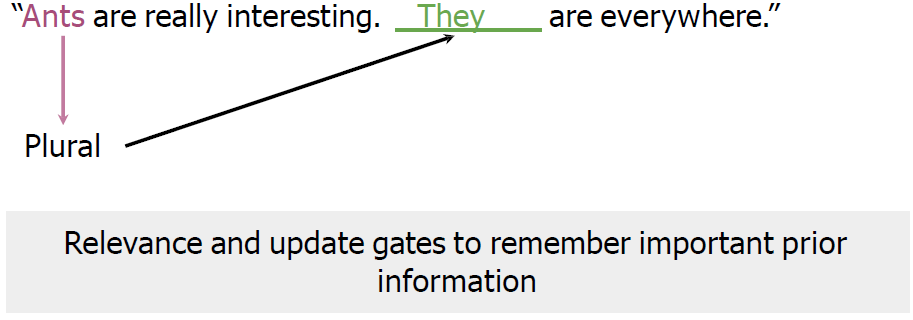
\includegraphics[width=\linewidth, height=0.9\textheight,keepaspectratio]{images/nlp/gru-1.png}
    \end{figure}

    \framebreak
    \begin{figure}
        \centering
        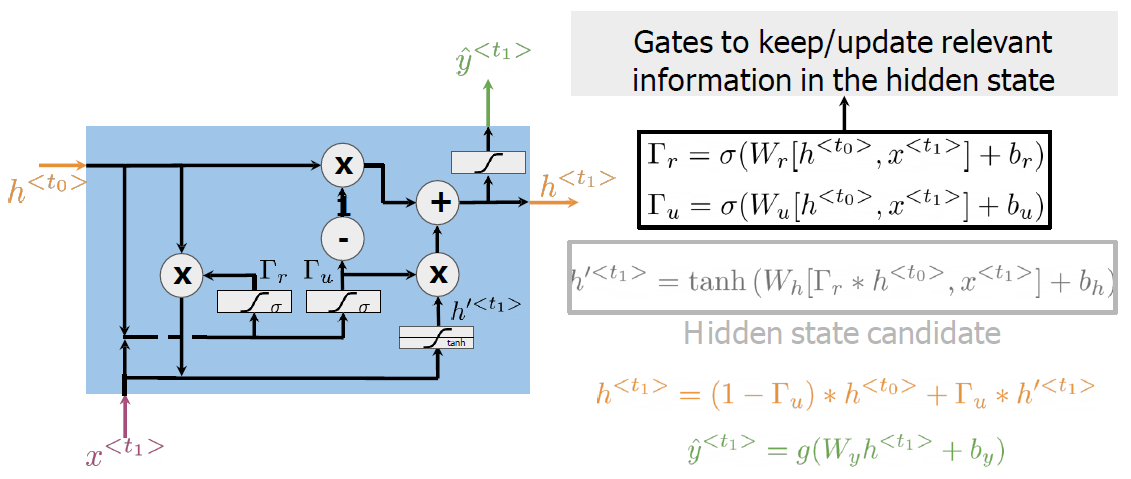
\includegraphics[width=\linewidth, height=0.9\textheight,keepaspectratio]{images/nlp/gru-2.png}
    \end{figure}
\end{frame}

\begin{frame}[allowframebreaks]{Vanilla RNN vsGRUs}
    \begin{figure}
        \centering
        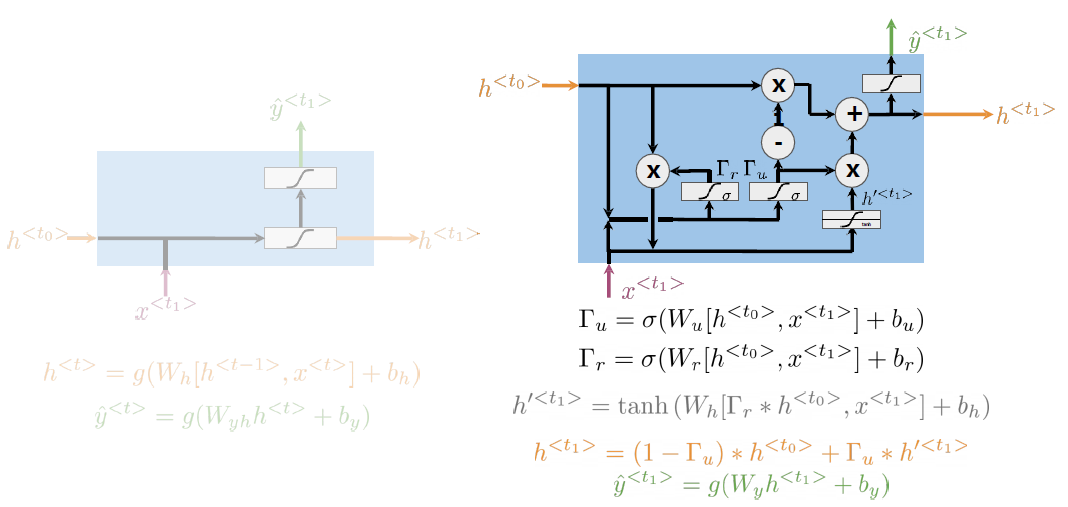
\includegraphics[width=\linewidth, height=0.9\textheight,keepaspectratio]{images/nlp/vanilla-rnn-vs-gru.png}
    \end{figure}
\end{frame}

\begin{frame}[allowframebreaks]{GRU: Key Properties}
    \begin{itemize}
        \item GRUs “decide” how to update the hidden state:
        \begin{itemize}
            \item The update gate controls the degree to which the hidden state is updated with new information.
            \item The reset gate determines how much of the previous hidden state to forget.
            \item This gating mechanism allows the GRU to adaptively capture dependencies of varying lengths.
        \end{itemize}
        \framebreak
        \item GRUs help preserve important information:
        \begin{itemize}
            \item By selectively updating and resetting, GRUs can retain relevant information over long sequences.
            \item This helps mitigate the vanishing gradient problem common in standard RNNs.
            \item As a result, GRUs are effective for tasks requiring memory of long-term context.
        \end{itemize}
    \end{itemize}
\end{frame}

\begin{frame}{Deep RNNs}
    \begin{figure}
        \centering
        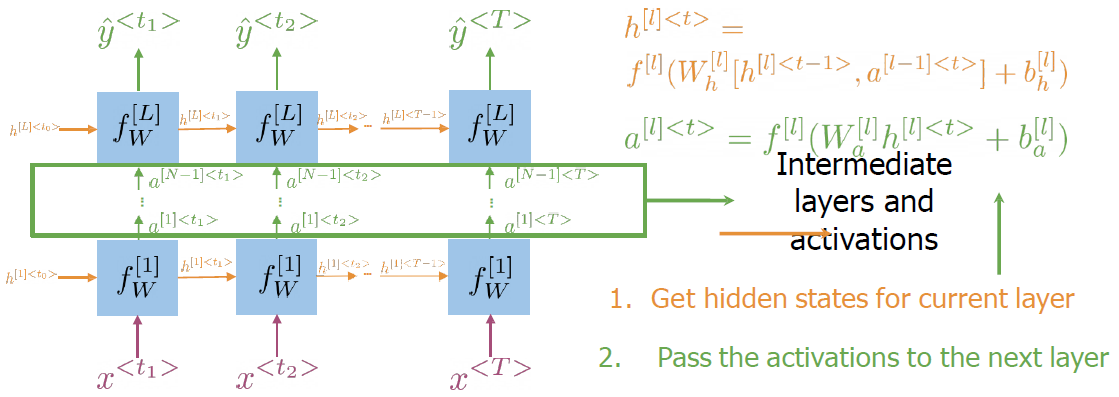
\includegraphics[width=\linewidth, height=0.9\textheight,keepaspectratio]{images/nlp/deep-rnn.png}
    \end{figure}

    Deep RNNs have more than one layer, which helps in complex tasks.
\end{frame}

\begin{frame}{RNNs: Advantages}
    \begin{itemize}
        \item Captures dependencies within a short range.
        \item Takes up less RAM than other n-gram models.
    \end{itemize}
\end{frame}

\begin{frame}{RNNs: Disadvantages}
    \begin{itemize}
        \item Struggles to capture long-term dependencies.
        \item Prone to vanishing or exploding gradients.
    \end{itemize}
\end{frame}

\begin{frame}{RNN Basic Structure}
    \begin{figure}
        \centering
        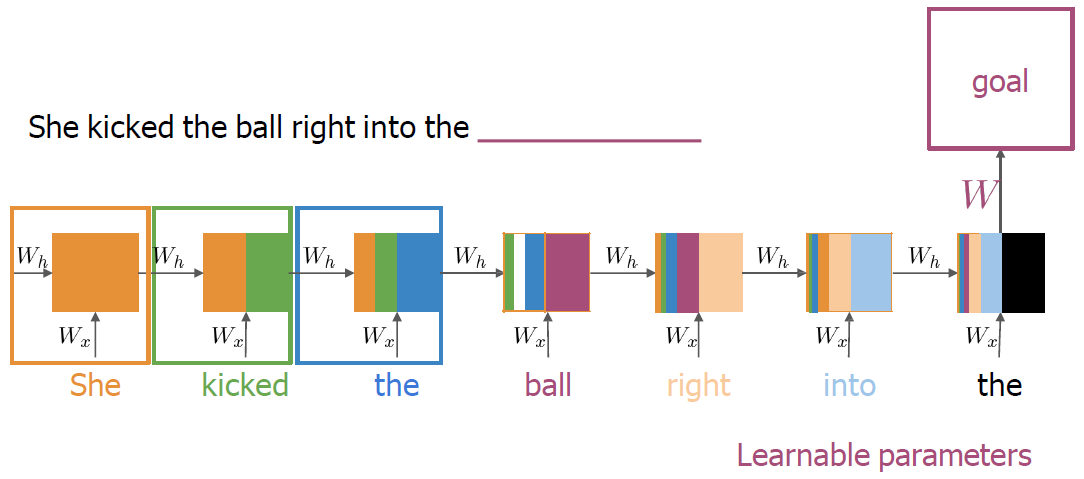
\includegraphics[width=\linewidth, height=0.9\textheight,keepaspectratio]{images/nlp/rnn-basic-structure.png}
    \end{figure}
\end{frame}

\begin{frame}[allowframebreaks]{Backpropagation Through Time (BPTT)}
    \begin{figure}
        \centering
        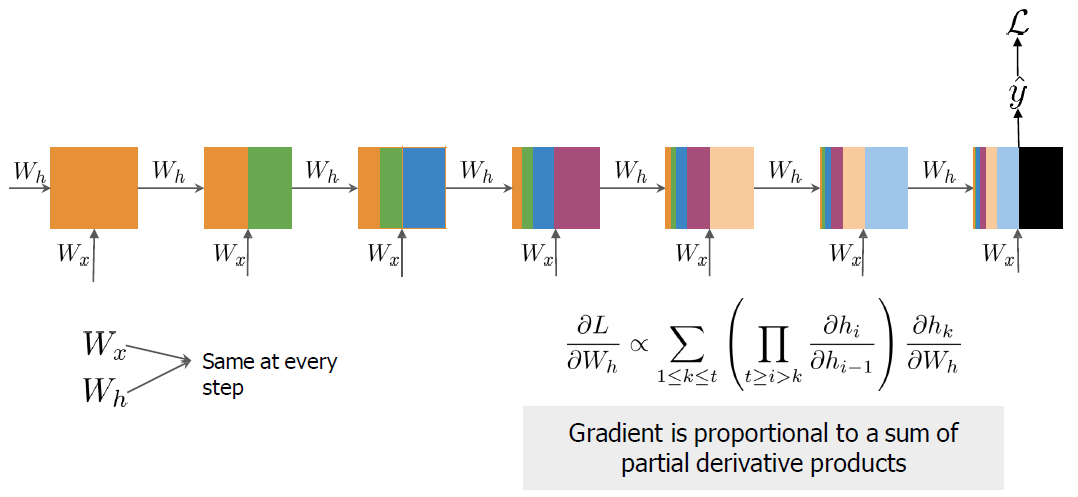
\includegraphics[width=\linewidth, height=0.9\textheight,keepaspectratio]{images/nlp/rnn-backpropagation.png}
    \end{figure}
    \framebreak
    \begin{figure}
        \centering
        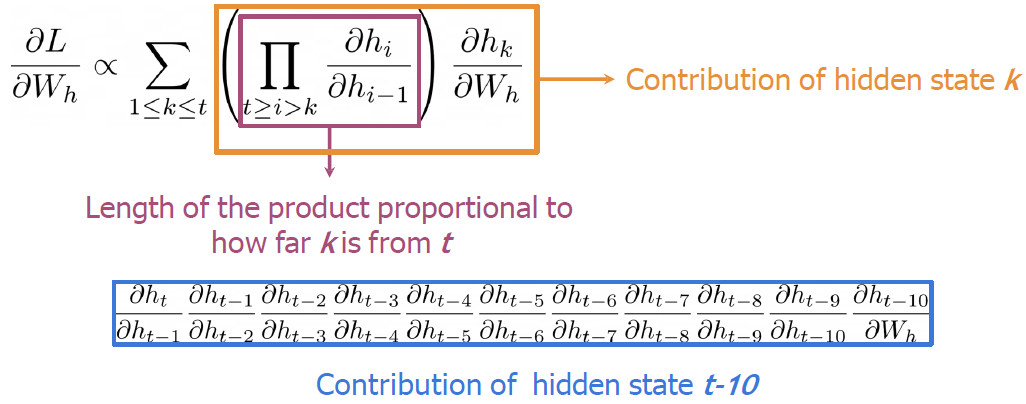
\includegraphics[width=\linewidth, height=0.9\textheight,keepaspectratio]{images/nlp/rnn-backpropagation-2.png}
    \end{figure}
\end{frame}

\begin{frame}{Solving for Vanishing or Exploding Gradients}
    \begin{figure}
        \centering
        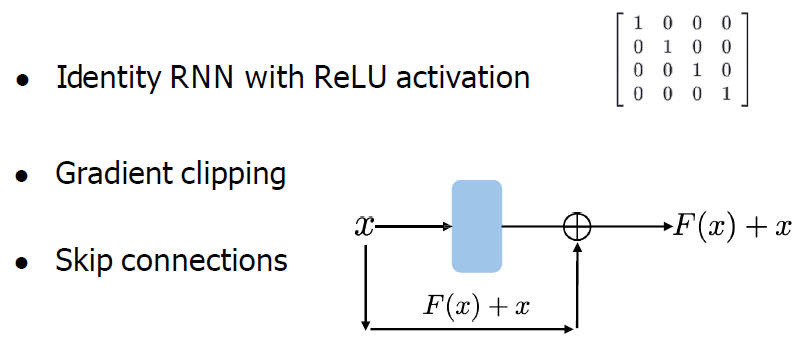
\includegraphics[width=\linewidth, height=0.9\textheight,keepaspectratio]{images/nlp/vanishing-exploding-gradients.png}
    \end{figure}
\end{frame}